% ===========================================================================
% DeepONet-Based Neural Network for Thomson Scattering Profile Fitting on EAST
% Target: Fusion Engineering and Design (FED, Elsevier) — 备选投稿版
% (由 PST 版 manuscript.tex 生成；PST 版请勿与本文档混用)
% ===========================================================================

\documentclass[a4paper,12pt]{article}

% ---- Packages ----
\usepackage{amsmath,amssymb}
\usepackage{graphicx}
\usepackage{booktabs}
\usepackage{multirow}
\usepackage{hyperref}
\usepackage[margin=2.5cm]{geometry}
\usepackage{caption}
\usepackage{subcaption}
\usepackage{microtype}
\microtypesetup{expansion=false}  % disable font expansion for compatibility
\usepackage{enumitem}

% Relaxed spacing for narrow columns
\sloppy
\hyphenpenalty=1000
\tolerance=2000

% ---- Metadata ----
\title{DeepONet-Based Neural Network for Thomson Scattering \\ Profile Fitting on EAST Tokamak}

\author{%
C.Y. Hu$^{a,b,c}$, Q. Zang$^{c,\ast}$\thanks{Corresponding author. E-mail address: zangq@ipp.ac.cn (Q. Zang).} \\[4pt]
$^a$ Anhui University of Science and Technology, Huainan 232001, China \\
$^b$ Institute of Energy, Hefei Comprehensive National Science Center \\
(Anhui Energy Laboratory), Hefei 230031, China \\
$^c$ Institute of Plasma Physics, Chinese Academy of Sciences, \\
Hefei 230031, China
}

\date{\today}

\begin{document}
\maketitle

% Highlights are submitted separately in the Editorial Manager system (3--5 bullets, <=85 chars each);
% they must NOT appear in the manuscript body (see paper/highlights.txt).

\begin{abstract}
\small
Thomson Scattering (TS) diagnostics on EAST measure electron temperature (Te) and density (ne) at 20--30 spatial channels; reconstructing continuous profiles is a prerequisite for transport and equilibrium analysis. The established modified hyperbolic tangent (mtanh) method relies on diagnostic-specific branches and hand-tuned parameters, limiting scalability to thousands of annual discharges. We propose a DeepONet-based neural network that replaces the seven-step mtanh pipeline with a single 14 ms forward pass, trained on (scattered points, mtanh-fitted profile) pairs from 161 EAST discharges. Five architectures are compared. ProfileNet, BiLSTM, Transformer, and CNN-DeepONet share one CoordDecoder trunk and one physics-constrained loss; a pure CNN-1D acts as a control. On 68 unseen test profiles (5 shots, 24 time points) spanning L-mode to strong H-mode (Te = 0.2--7.2 keV), the networks achieve mean absolute errors of Te = 0.34--0.51 keV, ne = 0.06--0.11 (10\textsuperscript{19} m\textsuperscript{-3}), and Ti = 0.07--0.14 keV relative to the mtanh baseline.

Ablation shows that removing the physics constraints improves ProfileNet ($-$11.8\%) and Transformer ($-$8.7\%) but degrades CNN-1D (+25.8\%) and LSTM (+30.6\%). The branch--trunk dot product confines outputs to smooth basis combinations---structural regularization for static encoders; the recurrent branch still needs explicit constraints. A per-profile Gaussian-process baseline is more accurate in-sample but 6--10$\times$ slower. A controlled CNN-DeepONet variant (CNN encoder plus shared trunk) resolves the confound: the trunk decoder improves Ti substantially (0.142 to 0.082 keV) but not Te or ne. No architecture is best for all diagnostics; we recommend a diagnostic-matched ensemble (CNN-Te + ProfileNet-ne + LSTM-Ti, total inference <50 ms).

\end{abstract}

\noindent\textbf{Keywords}: EAST tokamak, Thomson scattering, profile fitting, DeepONet, neural network, physics-constrained learning

% ===========================================================================
% 1. Introduction
% ===========================================================================
\section{Introduction}

The Experimental Advanced Superconducting Tokamak (EAST) at the Institute of Plasma Physics, Chinese Academy of Sciences (ASIPP), is a fully superconducting tokamak dedicated to long-pulse, high-performance plasma operation~\cite{east_overview}. Understanding the spatial structure of kinetic profiles---electron temperature $T_e(\rho)$, electron density $n_e(\rho)$, and ion temperature $T_i(\rho)$ as functions of the normalized minor radius $\rho$---is essential for transport analysis and equilibrium reconstruction. EAST's Thomson Scattering (TS) diagnostic measures $T_e$ and $n_e$ at $\sim$20--30 spatial channels~\cite{east_ts,east_tvts}, supplemented by a Reflectometer (Refl) for higher-resolution $n_e$ and an X-ray Crystal Spectrometer (TXCS) for $T_i$. These discrete scattered points must be reconstructed into continuous profiles before they can be used in codes such as ONETWO~\cite{onetwo} or TRANSP.

The standard profile fitting method on EAST employs a modified hyperbolic tangent (mtanh) function~\cite{mtanh_groebner}, which partitions the profile into a core spline region ($\rho < 0.85$) and a pedestal mtanh region ($\rho > 0.85$) connected by a smooth transition. The method is physically motivated and widely validated, but in practice it has real limitations. The pipeline is a seven-step chain (IQR outlier removal, core spline fitting, pedestal mtanh optimization, smooth transition, left-boundary correction) realized as six diagnostic-specific code branches. Every branch carries hand-tuned parameters (pedestal position, IQR thresholds, spline knots) that can fail on unusual discharges; every fit must be checked by eye; and the pedestal least-squares optimization is sensitive to its starting point. These issues limit scalability to EAST's annual output of thousands of discharges.

Machine learning has reached fusion diagnostics as well: Gaussian Process Regression for profile fitting~\cite{gpr_profiles,gpr_review}, Bayesian integrated data analysis~\cite{ida_east}, neural networks for TS temporal super-resolution~\cite{diag2diag}, and CNN-based density profile reconstruction~\cite{lan_cnn_east}. The Deep Operator Network (DeepONet)~\cite{deeponet} is a neural architecture specifically designed to learn mappings between function spaces, separating an operator $G: u \mapsto G(u)$ into a branch network encoding the input function and a trunk network encoding the output domain~\cite{physics_informed_deeponet,pinn_review}. The branch-trunk form has one property we rely on throughout: the output $\hat{y}(\rho) = \sum b_k \cdot t_k(\rho)$ is always a linear combination of smooth basis functions. Non-physical oscillations are excluded by construction, and we treat the architecture itself as \textit{structural regularization} for profile fitting.

In this work, we propose a DeepONet-based neural network that replaces the seven-step mtanh pipeline with a single $\sim$14 ms forward pass. Five architectures are compared---four (ProfileNet (SetEncoder), BiLSTM, Transformer, and CNN-DeepONet) share a common CoordDecoder and physics-constrained loss, while a pure CNN-1D serves as a control group without the branch-trunk structure---enabling a controlled study of architectural inductive biases. Our contributions include: (1) to the best of our knowledge, the first application of DeepONet to EAST TS profile fitting; (2) systematic five-architecture comparison under unified conditions; (3) a controlled CNN-DeepONet variant that resolves the encoder/decoder confound, showing the shared trunk decoder is beneficial for sparse diagnostics (Ti) but not dense ones (Te, ne); (4) ablation experiments showing that the branch-trunk structure regularizes static encoders by itself (without physics constraints ProfileNet and Transformer improve by 8--12\%, while CNN-1D and LSTM degrade by 26--31\%); (5) discovery of a diagnostic-architecture matching pattern reflecting intrinsic differences in diagnostic spatial sampling. In brief, the methodological novelty of this work lies in two intertwined ideas: treating the operator-learning structure itself as a built-in regularizer, and designing the comparison (shared trunk, controlled CNN-DeepONet variant, unified physics-constrained loss) so that this claim is testable rather than assumed.

% ===========================================================================
% 2. Method
% ===========================================================================
\section{Method}

\subsection{Problem Formulation}

Given $N$ discrete diagnostic measurements $\{(\rho_i, y_i)\}_{i=1}^N$, where $\rho_i \in [0, 1]$ is the normalized minor radius and $y_i$ is the physical quantity ($T_e$ in eV, $n_e$ in $10^{19}$ m$^{-3}$, or $T_i$ in keV), with $N$ typically ranging from 5 to 35 depending on the diagnostic, the goal is to learn a mapping $\mathcal{F}$ that outputs a smooth profile $\hat{y}(\rho)$ evaluated on a uniform grid of 201 points over $\rho \in [0, 1]$.

The mtanh approach implements $\mathcal{F}$ through an explicit parametric pipeline: IQR outlier removal $\to$ core spline fitting $\to$ pedestal mtanh parameter optimization $\to$ smooth transition $\to$ left-boundary correction. In contrast, the neural network approach learns $\mathcal{F}$ implicitly through supervised learning on a dataset of (scattered points, fitted profile) pairs.

\subsection{Training Data}

Training data were constructed from EAST discharges spanning 2015--2024 campaigns (161 shots, shot numbers 60150--149600). For each (shot, time) pair with available diagnostic data, the standard mtanh pipeline was executed to produce a 201-point fitted profile serving as the training label. The raw scattered diagnostic points---without IQR cleaning---serve as the neural network input. Invalid channels (non-finite readings or values below diagnostic-specific validity thresholds) are masked out when the scatter input is constructed; all encoders natively accept variable-length point sets, and CNN-1D additionally encodes the mask as a second input channel.

\textbf{H-mode/L-mode classification}: The energy confinement factor $H_{98}$ was read from the EAST MDSplus \texttt{energy\_east} tree ($\backslash$H98\_MHD signal). Time points with $H_{98} \geq 0.7$ are classified as H-mode, $0 < H_{98} < 0.7$ as L-mode, and $H_{98} = 0$ as unknown (data unavailable). The 0.7 threshold sits between typical L-mode confinement values and the nominal H-mode level ($H_{98}(y,2) \approx 1.0$); time points without a valid $H_{98}$ reading are excluded from mode-specific comparisons.

\textbf{Held-out test set}: To prevent data leakage, the test set consists exclusively of 2024 discharges outside the training shot range (60150--149600); no test data are used in training or validation. The train/validation split is 70/15/15. The test set consists of 5 unseen 2024 shots (156005, 156010, 156100, 156400, 156900) covering L-mode to strong H-mode conditions ($T_e = 0.2$--$7.2$ keV). Two further 2024 discharges were examined and excluded: 156200, because its EFIT equilibrium coverage ends at 10.6 s while the TS data span 32--101 s (unreliable $\rho$ mapping), and the last two time points of 156900 (discharge ramp-down, 7.5--8.5 s), whose mtanh reference profiles become non-physical. Key test set statistics are summarized in Table~\ref{tab:testset}.

\begin{table}[htbp]
\centering\footnotesize
\caption{Test set characteristics. All 5 shots are from the 2024 EAST campaign and are excluded from the training set. The $T_e$ range is the range of mtanh-fitted core $T_e$ across the shot's time points.}
\label{tab:testset}
\resizebox{\textwidth}{!}{%
\begin{tabular}{cccccccc}
\toprule
\textbf{Shot} & \textbf{Time Points} & \textbf{$T_e$ Range (keV)} & \textbf{Mode (H/L/unk)} & \textbf{$H_{98}$ Range} & \textbf{TS} & \textbf{Refl} & \textbf{TXCS} \\
\midrule
156005 & 2 & 2.3--2.4 & 1H / 1L & 0.69--0.96 & \checkmark & \checkmark & \checkmark \\
156010 & 6 & 0.2--2.0 & 6 unknown & 0.0$^*$ & \checkmark & \checkmark & \checkmark \\
156100 & 6 & 1.2--3.3 & 1H / 5L & 0.56--1.10 & \checkmark & \checkmark & \checkmark \\
156400 & 6 & 3.8--7.2 & 6H & 0.85--1.15 & \checkmark & \checkmark & \checkmark \\
156900 & 4 & 0.2--1.1 & 4L & 0.70$^{\dagger}$ & \checkmark & \checkmark & -- \\
\midrule
Total & 24 & 0.2--7.2 & 8H / 10L / 6unk & --- & 24 & 24 & 20 \\
\bottomrule
\end{tabular}%
}
\vspace{4pt}
\footnotesize{$^*$ Shot 156010: $H_{98}$ data unavailable from MDSplus (returns 0.0). Plasma mode is marked as ``unknown.'' $^{\dagger}$ Shot 156900: the $H_{98}$ signal ends at 2.53 s; the last available value (0.698) is used for all time points, giving L-mode classification. TXCS ($T_i$) data are not available for this shot.}
\end{table}

\subsection{Model Architecture}

Four of the five architectures share a common DeepONet-style decoder and differ only in the encoder design (Figure~\ref{fig:architecture}); the fifth, CNN-1D, uses a pure convolutional decoder as a control. The shared \textbf{CoordDecoder} (trunk net) is an MLP(1$\to$128$\to$128, SiLU) that maps the output coordinate $\rho$ to a set of basis functions $\mathbf{b}(\rho) \in \mathbb{R}^{128}$. The final output is:
\begin{equation}
\hat{y}(\rho) = \operatorname{Softplus}\left(\mathbf{z} \cdot \mathbf{b}(\rho)\right) = \operatorname{Softplus}\left(\sum_{k=1}^{128} z_k \cdot b_k(\rho)\right)
\label{eq:dotproduct}
\end{equation}
where $\mathbf{z} \in \mathbb{R}^{128}$ is the latent vector produced by the encoder. The Softplus activation ($\ln(1 + e^x)$) ensures positivity of the predicted physical quantities.

\begin{figure}[htbp]
\centering
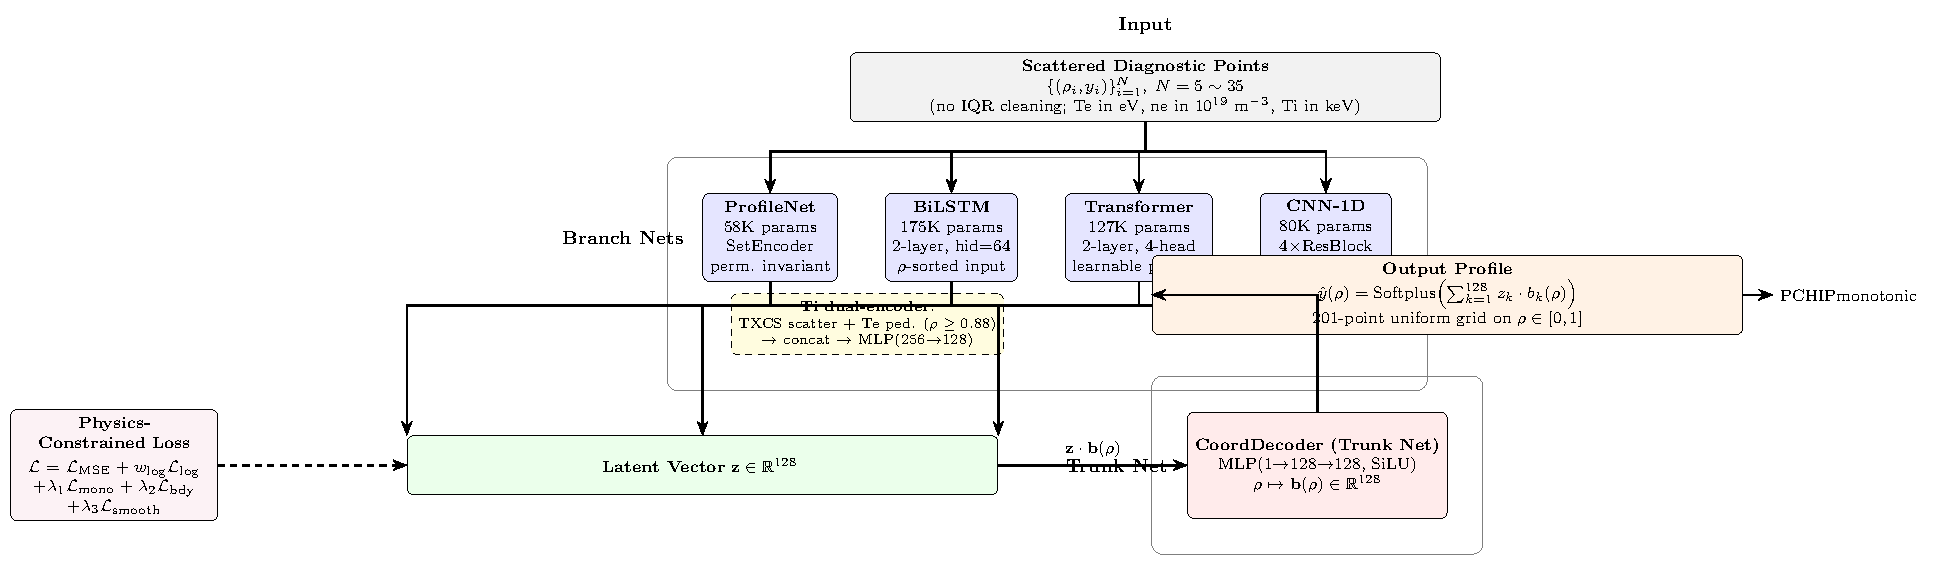
\includegraphics[width=\textwidth]{fig1_architecture.pdf}
\caption{DeepONet-based architecture for TS profile fitting. Four DeepONet encoder variants (branch nets)---ProfileNet, BiLSTM, Transformer, and CNN-DeepONet---encode scattered diagnostic points into a latent vector $\mathbf{z}$. A shared CoordDecoder (trunk net) maps the output coordinate $\rho$ to smooth basis functions $\mathbf{b}(\rho)$. The dot product $\mathbf{z}\cdot\mathbf{b}(\rho)$, followed by Softplus activation, produces the continuous profile $\hat{y}(\rho)$. A fifth architecture, CNN-1D, uses pure convolutional encoder--decoder layers without the branch-trunk structure, serving as a control group. Ti models use a dual-encoder design (TXCS scatter + Te pedestal). Training is supervised by a physics-constrained loss combining region-weighted MSE with monotonicity, boundary, and smoothness penalties.}
\label{fig:architecture}
\end{figure}

\begin{figure}[htbp]
\centering
\includegraphics[width=0.95\textwidth]{paper_results/figures/fig2_hmode_overlay.png}
\caption{Typical H-mode profile fitting results: six methods (mtanh baseline + five NN architectures) compared on three representative H-mode time points across Te, ne, and Ti diagnostics. The gray shaded band is the acceptance band (Section~\ref{sec:results}): its half-width follows the local dispersion of the diagnostic channels around the mtanh reference, and curves lying inside it are considered acceptable.}
\label{fig:hmode}
\end{figure}

In Figure~\ref{fig:hmode}, a good fit can be read off directly: the profile should pass through the core diagnostic channels, reproduce the mtanh baseline's overall shape, and---most importantly---track the steep pedestal gradient at $\rho = 0.85$--$1.0$, where H-mode physics information is concentrated; it should remain smooth, positive, and monotone, with no unphysical oscillations in the edge region, and it should stay inside the gray acceptance band where the diagnostic channels constrain it. Architectures that over-smooth the pedestal, oscillate near the edge, or leave the band score correspondingly worse on the MAE metrics of Table~\ref{tab:metrics} and the in-band fractions of Table~\ref{tab:band}.

\subsubsection{Encoder Architectures}

\textbf{ProfileNet (67K parameters)}: A PointNet-style SetEncoder~\cite{pointnet} with permutation-invariant max-pooling that processes each scattered point independently through an MLP, aggregates via max-pooling, and projects to $\mathbf{z}$. The architecture is permutation-invariant---the order of diagnostic points does not affect the output.

\textbf{LSTM (76K parameters)}: A single-layer bidirectional LSTM~\cite{lstm} (hidden=64) processes the scattered points sorted by $\rho$. The final forward and backward hidden states are concatenated and projected to $\mathbf{z}$. The BiLSTM captures sequential radial structure along the $\rho$-coordinate.

\textbf{Transformer (136K parameters)}: A 2-layer TransformerEncoder~\cite{transformer} (4-head self-attention, hidden=64) with learnable positional encodings processes sorted points. Self-attention allows each diagnostic channel to directly attend to any other channel, capturing global correlations.

\textbf{CNN-DeepONet (79K parameters)}: A CNN encoder---Conv1d stem, 3$\times$ ResidualBlock1D, and a global max-pool---that matches CNN-1D's encoder, but terminates in the shared CoordDecoder via the branch-trunk dot product. This variant was introduced to resolve a confound in the original comparison: CNN-1D differed from the other three models in \textit{both} encoder and decoder, so its inferior performance could not be attributed to either component alone. Pairing a CNN encoder with the shared trunk isolates the decoder's contribution.

\textbf{CNN-1D (66K parameters, control group)}: A pure 1D ResNet with 4$\times$ ResidualBlock1D. \textbf{This architecture intentionally does not use the DeepONet branch-trunk structure.} Instead, scattered points are linearly interpolated to a 201-point grid, stacked as a 2-channel tensor [values, mask], and processed through Conv1d encoder-decoder layers with residual connections. No BatchNorm is used. Together with CNN-DeepONet, this pair isolates the effect of the branch-trunk decoder under an otherwise identical CNN encoder.

\subsubsection{Ti Dual-Encoder}

All architectures use a dual-encoder design for $T_i$: one encoder processes the TXCS scattered points (main), while a second encoder processes $T_e$ pedestal data ($\rho \geq 0.88$). The two latent vectors are concatenated and fused via MLP(256$\to$128$\to$128). This design mirrors the mtanh practice of using $T_e$ pedestal information to constrain $T_i$ edge fitting.

\subsection{Physics-Constrained Loss Function}

The training objective combines a region-weighted MSE with physics-inspired auxiliary terms:

\begin{equation}
\mathcal{L} = \mathcal{L}_{\text{MSE}} + w_{\log} \mathcal{L}_{\log} + \lambda_1 \mathcal{L}_{\text{mono}} + \lambda_2 \mathcal{L}_{\text{bdy}} + \lambda_3 \mathcal{L}_{\text{smooth}}
\label{eq:loss}
\end{equation}

\begin{itemize}
    \item $\mathcal{L}_{\text{MSE}}$: Region-weighted MSE (core $\rho < 0.85$: 3$\times$, pedestal $\rho \geq 0.85$: 25$\times$), prioritizing accurate pedestal reconstruction.
    \item $\mathcal{L}_{\log}$ ($w_{\log}=0.1$): Log-space MSE, penalizing relative errors in low-value edge regions where absolute errors are naturally small but physically significant.
    \item $\mathcal{L}_{\text{mono}}$ ($\lambda_1=0.05$): $\operatorname{ReLU}(+d\hat{y}/d\rho)$, penalizing only positive derivatives, i.e., local non-monotonic increases in a profile that should decrease monotonically with $\rho$. Does not enforce global monotonicity; only suppresses local non-physical increases.
    \item $\mathcal{L}_{\text{bdy}}$ ($\lambda_2=0.05$): Minimizes $|d\hat{y}/d\rho|$ for $\rho < 0.05$, enforcing the magnetic axis symmetry condition $dT/d\rho|_{\rho=0} = 0$.
    \item $\mathcal{L}_{\text{smooth}}$ ($\lambda_3=0.01$): Penalizes large second derivatives $|d^2\hat{y}/d\rho^2|$, suppressing high-frequency oscillations.
\end{itemize}

The penalty weights ($\lambda_1$, $\lambda_2$, $\lambda_3$, $w_{\log}$) were set empirically on the validation set and are kept identical across all architectures to preserve comparability; their influence is examined directly in the ablation study (Table~\ref{tab:ablation}).

\subsection{Training Details}

All models are trained with AdamW optimizer (learning rate $10^{-3}$, weight decay $10^{-5}$), cosine annealing learning rate schedule, batch size 64, and a maximum of 500 epochs with early stopping (patience = 100). Post-inference, a PCHIP (Piecewise Cubic Hermite Interpolating Polynomial) shape-preserving interpolation is applied to enforce strict monotonic decrease and floor-value edge protection. All reported metrics are evaluated on the profiles after this post-processing step; we verified on the Te test points that the PCHIP step changes both the fit-to-scatter and the vs-mtanh MAE by less than 0.001 keV, i.e., it does not materially affect the reported numbers. Inference times are measured on CPU (10 warm-up runs followed by 200 timed passes through the full inference function, model loading excluded); the end-to-end speed comparison against the mtanh pipeline is reported in Section~\ref{sec:results}.

% ===========================================================================
% 3. Results
% ===========================================================================
\section{Results}
\label{sec:results}

\subsection{Fitting Accuracy: Five Architectures vs. mtanh}

Table~\ref{tab:metrics} presents the overall fitting accuracy of the five neural network architectures relative to the mtanh baseline across all 24 test time points (68 unique profiles; 340 NN profile predictions). The mean absolute error (MAE) is the primary metric. Because absolute errors are not directly comparable across plasma modes (the H-mode test shots reach $T_e$ up to 7.2 keV), mean relative errors (MeanRel\%) are reported by mode in the Appendix (Table~\ref{tab:meanrel}); RMSE and MaxAE, which exhibit the same architecture rankings as MAE, are available in the supplementary material (\texttt{paper\_results/all\_metrics.csv}).

\begin{table}[htbp]
\centering\footnotesize
\caption{Fitting accuracy (MAE $\pm$ std) of NN methods relative to mtanh baseline, by diagnostic and plasma mode. Lowest mean in each row is \textbf{bold}; bold does not imply statistical significance against adjacent values (see the paired Wilcoxon tests in Section~\ref{sec:results}). H-mode: 8 time points; L-mode: 10 time points; All: 24 time points (including 6 unknown-mode). The $\pm$ values are the standard deviation of MAE across the time points within each group (not measurement uncertainty). $T_i$ is evaluated on 20 time points (shot 156900 lacks TXCS data).}
\label{tab:metrics}
\resizebox{\textwidth}{!}{%
\begin{tabular}{c c | c c c c c}
\toprule
\textbf{Diag.} & \textbf{Mode} & \textbf{ProfileNet} & \textbf{LSTM} & \textbf{CNN-1D} & \textbf{CNN-DeepONet} & \textbf{Transformer} \\
\midrule
\multirow{3}{*}{Te (keV)}
    & All   & 0.512$\pm$0.283 & 0.347$\pm$0.194 & \textbf{0.342$\pm$0.292} & 0.393$\pm$0.328 & 0.350$\pm$0.317 \\
    & H     & 0.639$\pm$0.246 & \textbf{0.525$\pm$0.162} & 0.660$\pm$0.297 & 0.755$\pm$0.306 & 0.694$\pm$0.320 \\
    & L     & 0.298$\pm$0.206 & 0.224$\pm$0.125 & 0.206$\pm$0.080 & 0.199$\pm$0.063 & \textbf{0.185$\pm$0.073} \\
\midrule
\multirow{3}{*}{$n_e$ (10$^{19}$)}
    & All   & \textbf{0.057$\pm$0.018} & 0.060$\pm$0.018 & 0.067$\pm$0.023 & 0.075$\pm$0.020 & 0.112$\pm$0.025 \\
    & H     & \textbf{0.058$\pm$0.014} & 0.065$\pm$0.022 & 0.067$\pm$0.032 & 0.073$\pm$0.021 & 0.120$\pm$0.021 \\
    & L     & \textbf{0.058$\pm$0.022} & 0.063$\pm$0.017 & 0.068$\pm$0.021 & 0.071$\pm$0.019 & 0.110$\pm$0.031 \\
\midrule
\multirow{3}{*}{$T_i$ (keV)}
    & All   & 0.091$\pm$0.048 & \textbf{0.074$\pm$0.039} & 0.141$\pm$0.047 & 0.082$\pm$0.044 & 0.089$\pm$0.062 \\
    & H     & 0.097$\pm$0.036 & \textbf{0.075$\pm$0.027} & 0.110$\pm$0.036 & 0.076$\pm$0.019 & 0.090$\pm$0.045 \\
    & L     & 0.073$\pm$0.066 & 0.046$\pm$0.028 & 0.150$\pm$0.037 & 0.054$\pm$0.018 & \textbf{0.041$\pm$0.018} \\
\bottomrule
\end{tabular}%
}
\end{table}

Key observations from Table~\ref{tab:metrics}:

\begin{enumerate}
    \item \textbf{No single architecture dominates all diagnostics.} CNN-1D (0.342 keV), LSTM (0.347 keV), and Transformer (0.350 keV) are statistically indistinguishable for Te; ProfileNet is significantly worse than LSTM, CNN-1D, and Transformer ($p<0.05$). For $T_i$, LSTM's lead (0.074 keV) is not significant against the other DeepONet variants ($p>0.15$), but all four significantly beat CNN-1D (0.141 keV, $p<0.01$). For $n_e$, ProfileNet (0.057) and LSTM (0.060) are indistinguishable ($p=0.08$), and both significantly beat CNN-1D ($p<0.05$) and Transformer (0.112, $p<0.001$). Encoder choice, it seems, interacts with how each diagnostic samples space; no single architecture is better everywhere.

    \item \textbf{L-mode accuracy exceeds H-mode for Te.} The H-mode Te MAE (0.525--0.694 keV) is consistently higher than L-mode Te MAE (0.185--0.298 keV). This is because the H-mode test set includes shot 156400 with very high core temperatures (up to 7.2 keV) and steep pedestals, amplifying absolute differences between mtanh and NN fits. In relative terms, H-mode errors (33--57\%) are lower than L-mode errors (43--97\%); the L-mode MeanRel\% is inflated by the newly added low-$T_e$ points of shot 156900 (core $T_e$ 0.2--1.1 keV), whose edge values approach zero and make relative error ill-conditioned (Table~\ref{tab:meanrel}).

    \item \textbf{The CNN-DeepONet control resolves the encoder/decoder confound.} Keeping the CNN encoder fixed and swapping CNN-1D's pure convolutional decoder for the shared CoordDecoder trunk improves $T_i$ sharply (0.141 to 0.082 keV, $-$42\%), while Te (0.342 to 0.393 keV) and $n_e$ (0.067 to 0.075) get slightly worse. The trunk helps exactly where the data are sparse---the 5--15 irregular TXCS channels---and does nothing where they are dense. For TS and Refl the data already fix the local shape, so a convolutional decoder is enough. CNN-1D's $T_i$ weakness is thus a property of its decoder, not its encoder.

    \item \textbf{Transformer excels in L-mode.} Transformer achieves the lowest L-mode MAE for both Te (0.185 keV) and $T_i$ (0.041 keV); these leads are not statistically significant at this sample size (Wilcoxon $p>0.05$), so the finding is suggestive of a genuine advantage of global self-attention on the smoother, less pedestal-dominated L-mode profiles, rather than established.
\end{enumerate}

To separate real differences from sampling noise, we ran paired Wilcoxon signed-rank tests on the per-time-point MAE within each (diagnostic, mode) group. The statistically robust findings are: (i) ProfileNet is significantly worse than LSTM, CNN-1D, and Transformer for Te ($p=0.001$--$0.04$); (ii) CNN-1D is significantly worse than the DeepONet variants for $T_i$ ($p<0.01$); (iii) Transformer is significantly worse than all other architectures for $n_e$ ($p<0.01$); and (iv) the CNN-DeepONet trunk swap improves $T_i$ significantly ($p<0.001$). All remaining rank differences are within sampling noise at the current test-set size.

Figure~\ref{fig:boxplot} shows the MAE distribution across all test time points as box plots, confirming the trends observed in Table~\ref{tab:metrics}.

\begin{figure}[htbp]
\centering
\includegraphics[width=0.85\textwidth]{paper_results/figures/fig6_mae_boxplot.png}
\caption{MAE distribution across all 24 test time points (vs. mtanh baseline). Each box shows median, quartiles, and outliers; means are annotated.}
\label{fig:boxplot}
\end{figure}

\subsubsection{Comparison with Gaussian Process Regression}

Gaussian process regression (GPR) is the established ML alternative for profile fitting, and a natural question is how the DeepONet compares. We fit a per-profile GPR (RBF kernel with white noise, hyperparameters optimized per profile by marginal likelihood) directly to the raw diagnostic scatter of each test point, and compare the fit-to-scatter MAE with the mtanh fit and with the stored ProfileNet profile (Table~\ref{tab:gpr}). This comparison is deliberately asymmetric: GPR is a non-parametric model evaluated in-sample on the very points it fits, whereas the NN is trained offline to reproduce the mtanh reference and never sees the test scatter; the fit-to-scatter objective is therefore GPR's home ground.

\begin{table}[htbp]
\centering\footnotesize
\caption{Fit-to-scatter MAE (mean $\pm$ std, interpolated to the raw diagnostic channel positions): per-profile RBF Gaussian process regression vs. the mtanh fit and the stored ProfileNet profile. GPR hyperparameters are optimized per profile; fit times are per profile on CPU.}
\label{tab:gpr}
\begin{tabular}{l c c c c}
\toprule
\textbf{Diagnostic} & \textbf{GPR} & \textbf{mtanh} & \textbf{ProfileNet} & \textbf{GPR fit time} \\
\midrule
Te (keV)       & 0.559$\pm$0.577 & 0.687$\pm$0.384 & 0.916$\pm$0.457 & 112--150 ms \\
$n_e$ (10$^{19}$) & 0.282$\pm$0.106 & 0.327$\pm$0.118 & 0.432$\pm$0.092 & $\sim$86 ms \\
$T_i$ (keV)    & 0.094$\pm$0.036 & 0.142$\pm$0.081 & 0.158$\pm$0.080 & $\sim$131 ms \\
\bottomrule
\end{tabular}
\end{table}

GPR achieves the lowest fit-to-scatter MAE on all three diagnostics: 19\% better than mtanh for Te ($p=0.10$, not significant), 14\% better for $n_e$ ($p=0.002$), and 34\% better for $T_i$ ($p<0.001$). The DeepONet's fit-to-scatter error is the largest because that is not its training objective---it reproduces the mtanh reference---and because the raw scatter contains invalid high-value channels (e.g., 15 keV sentinel readings) that the mtanh pipeline and the NN mask or reject but that dominate this metric. The trade-off is clear: GPR costs 86--150 ms per profile (6--10$\times$ the NN's 14--19 ms) with $O(N^3)$ scaling, requires per-profile hyperparameter optimization, and transfers nothing across discharges; the DeepONet provides uniform 14--19 ms inference, learns a dataset-level prior over 161 discharges, and generalizes without re-optimization. For bulk EAST processing---thousands of time points per campaign---the NN's latency and determinism dominate the comparison; for single high-value profiles where per-shot accuracy against the raw channels matters and a specialist can inspect the fit, GPR remains the better tool.

\subsection{H-mode vs. L-mode: Cross-Regime Robustness}

Figure~\ref{fig:hl} compares H-mode and L-mode MAE for each diagnostic-method combination. The neural networks demonstrate consistent performance across plasma regimes, with LSTM and Transformer showing the most balanced H/L accuracy profiles. The L-mode group now includes the low-$T_e$ discharge 156900 (core $T_e$ down to 0.2 keV), which extends the comparison to colder L-mode conditions than the original four shots.

\begin{figure}[htbp]
\centering
\includegraphics[width=0.90\textwidth]{paper_results/figures/fig7_hl_comparison.png}
\caption{H-mode vs. L-mode MAE comparison for each diagnostic and architecture. H-mode profiles (solid bars) correspond to $H_{98} \geq 0.7$; L-mode (hatched bars) to $0 < H_{98} < 0.7$.}
\label{fig:hl}
\end{figure}

\subsection{Pedestal Region Fitting}

The pedestal region ($\rho = 0.85$--$1.0$) is the most challenging part of H-mode profile fitting due to the steep gradient. Figure~\ref{fig:pedestal} shows a focused zoom of the Te pedestal region for representative H-mode time points. The NN methods generally track the mtanh pedestal shape well, though some architectures (particularly CNN-1D) show systematic deviations in the extreme edge region $\rho > 0.95$, where diagnostic measurements become sparse and noisy.

\begin{figure}[htbp]
\centering
\includegraphics[width=0.95\textwidth]{paper_results/figures/fig4_pedestal_zoom.png}
\caption{Pedestal region zoom ($\rho = 0.85$--$1.0$) for Te, showing all six methods on representative H-mode time points. The vertical dotted line at $\rho = 0.95$ marks the approximate separatrix position.}
\label{fig:pedestal}
\end{figure}

\subsection{Core Peakedness}

The core-to-edge peaking factor (peakedness $= y_{\text{core}} / y_{\text{edge}}$) is a key parameter for transport model validation. Figure~\ref{fig:peakedness} shows a scatter plot of NN-predicted peakedness versus mtanh reference peakedness across all test time points. Pearson correlation coefficients exceed 0.95 for all architecture-diagnostic combinations, indicating that while the NN methods may differ from mtanh in absolute profile values, they faithfully reproduce the relative core-to-edge peaking structure.

\begin{figure}[htbp]
\centering
\includegraphics[width=0.95\textwidth]{paper_results/figures/fig5_peakedness_scatter.png}
\caption{Core peakedness ($y_{\text{core}} / y_{\text{edge}}$): NN predictions vs. mtanh reference. Each point represents one time point, colored by shot. The diagonal dashed line indicates perfect agreement; Pearson $r$ values are annotated.}
\label{fig:peakedness}
\end{figure}

\subsection{Ablation Study: Physics Constraints vs. Architecture}

To decouple the contributions of the physics-constrained loss function from the architectural inductive bias, we conducted an ablation experiment: four architectures were retrained for Te with pure MSE loss ($\lambda_1 = \lambda_2 = \lambda_3 = w_{\log} = 0$), and compared with the original physics-constrained models. Results are shown in Table~\ref{tab:ablation}. (The CNN-DeepONet variant was added after this ablation was completed; its physics-off counterpart is deferred to future work.)

\begin{table}[htbp]
\centering\small
\caption{Ablation experiment results (Te diagnostic): MAE with and without physics constraints. $\Delta =$ (mean Physics-off MAE $-$ mean Physics-on MAE) / mean Physics-on MAE, averaged over the 24 test time points. Positive $\Delta$ indicates degradation when constraints are removed.}
\label{tab:ablation}
\begin{tabular}{lccc}
\toprule
\textbf{Architecture} & \textbf{Physics-on MAE} & \textbf{Physics-off MAE} & \textbf{$\Delta$} \\
\midrule
ProfileNet (DeepONet)   & 0.512 & 0.452 & \textbf{$-$11.8\%} (improved) \\
LSTM (DeepONet)         & 0.347 & 0.453 & \textbf{+30.6\%} (degraded) \\
CNN-1D (no DeepONet)    & 0.342 & 0.430 & \textbf{+25.8\%} (degraded) \\
Transformer (DeepONet)  & 0.349 & 0.318 & \textbf{$-$8.7\%} (improved) \\
\bottomrule
\end{tabular}
\end{table}

The ablation results split into three behaviors. The pooling- and attention-based DeepONets improve slightly when the physics constraints are removed (ProfileNet $-11.8\%$, Transformer $-8.7\%$); CNN-1D, which has no branch-trunk structure, degrades by $+25.8\%$; and LSTM degrades even more ($+30.6\%$, with H-mode MAE rising from 0.525 to 0.805 keV) despite sharing the same trunk. The DeepONet operator approximation theorem~\cite{deeponet} explains the first part: each basis function $t_k(\rho)$ is a smooth MLP output, so every linear combination $\sum b_k \cdot t_k(\rho)$ is $C^\infty$ smooth and high-frequency oscillations are excluded without any penalty, and the branch network can only select coefficients $b_k$, not independently modify each $\hat{y}(\rho_i)$. This structural regularization is sufficient for the static encoders, whose slight improvement without constraints further suggests that $\mathcal{L}_{\text{mono}} + \mathcal{L}_{\text{bdy}} + \mathcal{L}_{\text{smooth}}$ may slightly over-regularize them. The recurrent branch, however, is not fully tamed by the trunk: although every trunk output is smooth, unconstrained training lets the LSTM select large, noise-fitting coefficient combinations, so the physics penalties remain the effective regularizer for the recurrent encoder.

\subsection{Engineering Value: Speed, Automation, and Acceptance}

\textbf{Inference speed and determinism.} All five architectures achieve inference under $\sim$20 ms on a single CPU core (ProfileNet $\sim$15 ms, LSTM $\sim$14 ms, CNN-1D $\sim$16 ms, CNN-DeepONet $\sim$16 ms, Transformer $\sim$19 ms), making them suitable for both offline batch processing and potential real-time applications. For reference, we timed the mtanh pipeline end-to-end on the same CPU over the 24 test points: 16--71 ms per Te profile (median 36 ms), 16--870 ms for $n_e$ (median 30 ms; slow least-squares convergence produces the long tail), and $\sim$1 ms for $T_i$ (its parametric fit is lighter than the NN). The NN is thus 2--3$\times$ faster than mtanh for Te, faster in the slow-convergence cases for $n_e$, and slower than mtanh for $T_i$ in raw latency. The practical gain is therefore not raw speed but uniformity: one deterministic 14--19 ms pass with no per-case optimizer failure modes and no manual inspection. The diagnostic-optimal ensemble (CNN-based $T_e$ + ProfileNet-based $n_e$ + LSTM-based $T_i$, 66K+67K+76K parameters) runs under 50 ms combined.

\textbf{Automation and robustness.} Replacing the seven-step pipeline with a single forward pass removes the main scalability bottleneck: every mtanh fit must currently be checked by eye, and the pedestal least-squares optimization occasionally fails or converges to non-physical solutions that must be identified manually. The NN pipeline needs no such inspection---its output is smooth, positive, and (after the PCHIP step) monotone by construction, even for inputs outside the training distribution, so failures degrade gracefully rather than catastrophically. Invalid or missing diagnostic channels are handled by the same masking used in training, with no code-branch changes, and the scripted training pipeline allows the models to be periodically retrained as new campaigns accumulate. These properties matter at EAST's throughput of thousands of discharges per campaign, where manual inspection is the current rate-limiting step.

\textbf{An acceptance-band criterion.} To give the qualitative comparison of Figure~\ref{fig:hmode} a quantitative reading, we introduce a data-driven acceptance band around the mtanh reference: for each time point, the band half-width is the local median of $|y_{\text{scatter}} - y_{\text{mtanh}}|$ over the diagnostic channels (binned in $\rho$, floored at 0.05 in profile units), so the band represents the intrinsic dispersion of the diagnostic around the reference rather than an arbitrary tolerance. A fitted curve is considered acceptable where it lies inside this band. Table~\ref{tab:band} reports the mean in-band fraction over all test points. The evaluation reproduces the MAE rankings of Table~\ref{tab:metrics}---LSTM and Transformer lead for Te and Ti, and Transformer's weakness on $n_e$ is stark (11\% in-band)---while adding an interpretable, per-profile acceptance criterion applicable to every discharge in bulk processing without human inspection. The representative points shown in Figure~\ref{fig:hmode} were additionally screened by an automated quality check (non-finite values, non-monotone spikes, and far-outside-band deviations), so no obviously anomalous curves appear in the figure.

\begin{table}[htbp]
\centering\footnotesize
\caption{Acceptance-band evaluation: mean in-band fraction (\% $\pm$ std) of the fitted profile inside the scatter-derived band around the mtanh reference, over all test time points. Best per row in \textbf{bold}.}
\label{tab:band}
\begin{tabular}{l c c c c c}
\toprule
\textbf{Diag.} & \textbf{ProfileNet} & \textbf{LSTM} & \textbf{CNN-1D} & \textbf{CNN-DeepONet} & \textbf{Transformer} \\
\midrule
Te & 57.9$\pm$19.8 & 66.8$\pm$18.6 & 67.1$\pm$25.8 & 59.8$\pm$27.1 & \textbf{69.7$\pm$23.6} \\
$n_e$ & 53.3$\pm$20.0 & 47.2$\pm$15.8 & \textbf{55.5$\pm$7.4} & 36.9$\pm$12.7 & 11.1$\pm$15.1 \\
$T_i$ & 69.4$\pm$29.2 & \textbf{78.9$\pm$23.6} & 48.5$\pm$17.2 & 75.3$\pm$16.6 & 68.9$\pm$28.8 \\
\bottomrule
\end{tabular}
\end{table}

% ===========================================================================
% 4. Discussion
% ===========================================================================
\section{Discussion}

\subsection{Architecture as Regularization}

The ablation in Table~\ref{tab:ablation} shows that the branch-trunk structure and the physics loss are not interchangeable regularizers. In a DeepONet, the branch network only picks the coefficients $b_k$; the output must stay in the span of the trunk's smooth basis functions $\{t_k(\rho)\}$, so high-frequency oscillations are excluded by construction, much like the smoothness prior in Gaussian-process profile fits~\cite{gpr_profiles,gpr_review}, but without any tuning parameter. For the static encoders (ProfileNet's max-pooling, Transformer's self-attention) this structural smoothness alone suffices---removing the physics penalties even helps slightly. CNN-1D's decoder, by contrast, produces independent outputs at each $\rho_i$; without explicit penalties, nothing prevents non-physical profiles. LSTM occupies an intermediate but informative position: it shares the trunk, so its outputs are smooth by construction, yet removing the penalties still degrades it (+30.6\%, most strongly in H-mode), because the recurrent branch is free to select large, noise-fitting coefficient combinations. The trunk constrains the \textit{form} of the output; the physics penalties additionally constrain the \textit{coefficient dynamics} learned by the branch---and only some encoders need the latter. The same mechanism explains why the trunk helps sparse diagnostics (TXCS, 5--15 points) but not dense ones (TS, 20--30 points): where channels are dense, local continuity is already determined by the data and the convolutional decoder's locality suffices; where they are sparse, the basis-function subspace acts as a prior that fills the gaps between channels. When EAST data are processed in bulk, nobody can inspect every output; the guarantee that DeepONet profiles cannot oscillate wildly is then the main practical advantage.

\subsection{Diagnostic-Architecture Matching}

Table~\ref{tab:metrics} shows that no single architecture is optimal across all three diagnostics. We attribute this to how the three diagnostics sample space, not to differences in model capacity. TS gives 20--25 dense, evenly spaced channels, and CNN-1D's local kernels exploit that locality. Refl samples $n_e$ on an irregular, edge-concentrated grid of $\rho$ positions, where ProfileNet's permutation-invariant set pooling is the most robust. TXCS gives only 5--15 sparse, irregularly placed points, and there BiLSTM's gated sequence modeling is the most robust. The CNN-DeepONet control isolates the decoder's contribution directly: for sparse TXCS data, swapping CNN-1D's convolutional decoder for the shared trunk cuts $T_i$ MAE by 42\%; for dense TS/Refl data the trunk yields no improvement. The slight degradation on the dense diagnostics (Te 0.342$\to$0.393 keV, $n_e$ 0.067$\to$0.075) suggests that the trunk's 128-basis subspace, combined with the positivity-preserving Softplus output, slightly over-smooths the sharp pedestal features that dense local data resolve---the price of the same structural guarantee that pays off for sparse inputs. The trunk's smoothing, then, matters for sparse inputs and is redundant (mildly costly) where local continuity already holds. In practice we recommend a diagnostic-matched ensemble (CNN-based $T_e$ + ProfileNet-based $n_e$ + LSTM-based $T_i$, combined inference $<$50 ms); this reaches the best accuracy per diagnostic without asking for one universal architecture.

\subsection{Limitations and Outlook}

Several limitations should be noted. (1) $T_i$ training data is sparse ($\sim$148 vs. $\sim$342 for $T_e$) due to limited TXCS coverage in pre-2023 campaigns; the dual-encoder design partially compensates, but more data would benefit all architectures. (2) The NN models are trained with mtanh-fitted profiles as labels. A concept-validation experiment on the Te test points showed that direct scatter-MSE training yields slightly worse fit-to-scatter accuracy than mtanh-label training (mean MAE 0.953 vs. 0.916 keV) and, as expected, a worse reproduction of the mtanh reference; both approaches show 33--39\% higher MAE against the raw diagnostic points than the mtanh fit itself (0.687 keV). The NN models are therefore ``fast approximations to mtanh,'' not replacements. (3) ONETWO transport validation was prevented by ZFIT atomic physics incompatibility. (4) Test shots are limited to the 2024 campaign (6,405-shot gap from training data), with 10 L-mode time points; the added L-mode discharge 156900 lacks TXCS data ($T_i$ not evaluated on it), and its $H_{98}$/EFIT coverage ends before the diagnostic times, so its mode is assigned from the last available $H_{98}$ value and its $\rho$ mapping uses the last available equilibrium (up to 6 s earlier). (5) Unlike GPR methods~\cite{gpr_profiles,gpr_review}, the current models lack uncertainty quantification, which could be addressed via Monte Carlo Dropout or Deep Ensemble methods.

Neural operators are an active direction in fusion plasma modeling. Fourier Neural Operators have been demonstrated as plasma surrogates achieving multi-order-of-magnitude speedups~\cite{fno_plasma}, DeepONet architectures have been applied to equilibrium reconstruction~\cite{deeponet_equilibrium}, PINNs have been used for tokamak inverse problems~\cite{pinn_tokamak,pinn_east}, and neural network surrogates for kinetic EFIT have achieved real-time capable speeds~\cite{nn_efit_surrogate}. Combined with the present work on profile fitting, these approaches collectively suggest a pathway toward fully ML-driven plasma analysis workflows.

From an engineering standpoint, deploying the diagnostic-matched ensemble in EAST's automated processing raises several practical considerations. (i) \textit{Model updates}: the training pipeline is fully scripted, so the ensemble can be periodically retrained on the accumulating (scatter, mtanh-label) pairs of each new campaign at modest CPU cost. (ii) \textit{Abnormal discharges}: invalid channels are handled by the same masking used in training; even for inputs far outside the training distribution, the branch-trunk output remains smooth, positive, and monotone after the PCHIP step---a guarantee the hand-tuned pipeline cannot make---so failures are graceful rather than catastrophic. (iii) \textit{Diagnostic robustness}: because every encoder accepts variable-length masked point sets, missing or failed TS/Refl/TXCS channels require no code-branch changes, unlike the six diagnostic-specific mtanh paths. (iv) \textit{Integration}: the inference functions are self-contained PyTorch CPU modules that take the same (rho, value) arrays already produced by the existing MDSplus readers, and the ensemble latency ($<$50 ms per profile) is compatible with inter-shot processing cadence.

% ===========================================================================
% 5. Conclusion
% ===========================================================================
\section{Conclusion}

We have presented a DeepONet-based neural network framework for Thomson Scattering profile fitting on EAST, replacing the traditional seven-step mtanh pipeline with a single 14 ms forward pass. Five architectures were systematically compared on 68 unique test profiles (24 time points across 5 unseen shots, 340 NN profile predictions) spanning L-mode to strong H-mode conditions: four encoder variants sharing a common CoordDecoder, plus a pure CNN-1D control without the branch-trunk structure.

Key findings include:

\begin{enumerate}
    \item \textbf{Fitting accuracy}: NN methods achieve MAE of $T_e = 0.34$--$0.51$ keV, $n_e = 0.06$--$0.11 \times 10^{19}$ m$^{-3}$, and $T_i = 0.07$--$0.14$ keV relative to mtanh, with smooth temporal trajectories and high core-peakedness correlation ($r > 0.95$).

    \item \textbf{Architecture matters more than loss design}: Ablation experiments show the branch-trunk dot product acts as a regularizer for static encoders: removing the physics constraints improves ProfileNet ($-$11.8\%) and Transformer ($-$8.7\%) but degrades CNN-1D (+25.8\%) and LSTM (+30.6\%). For scientific ML, that is a practical lesson about matching architecture and loss to the encoder family.

    \item \textbf{Diagnostic-architecture matching}: No single encoder is optimal for all diagnostics. The recommended deployment ensemble (CNN-based $T_e$ + ProfileNet-based $n_e$ + LSTM-based $T_i$) reflects intrinsic differences in diagnostic spatial sampling patterns. A controlled CNN-DeepONet variant confirms that the trunk decoder's regularization is diagnostic-specific: it improves sparse TXCS $T_i$ by 42\% while offering no benefit for dense TS/Refl diagnostics.

    \item \textbf{Engineering value}: the NN pipeline removes manual inspection and per-case optimizer failures, runs at uniform deterministic 14--19 ms latency (2--3$\times$ faster than mtanh for $T_e$), degrades gracefully under missing or invalid channels, and pairs with a data-driven acceptance-band criterion (Table~\ref{tab:band}) that flags unacceptable fits automatically---a practical basis for bulk-processing thousands of discharges per campaign without human intervention.

    \item \textbf{Positioning}: The NN models are fast, automated approximations to mtanh, not replacements for its accuracy. Their value is operational: thousands of discharges can be processed without manual intervention, at some cost in fitting precision relative to mtanh.
\end{enumerate}

Future work will focus on: (a) expanding $T_i$ and L-mode training data with 2024--2025 EAST campaigns; (b) resolving ONETWO transport code compatibility to enable full-pipeline physics validation; (c) adding uncertainty quantification via ensemble methods; (d) deploying the diagnostic-matched ensemble to EAST's automated data processing workflow; and (e) exploring the transfer of this framework to other tokamaks with similar diagnostic configurations.

% ===========================================================================
% Acknowledgments
% ===========================================================================
\section*{Acknowledgments}

The authors thank the EAST team for diagnostic data access and operational support. This work is supported by the National Natural Science Foundation of China under Grant No. 12135015, and the National MCF Energy R\&D Program under Grant No. 2025YFE03050001.

% ===========================================================================
% Appendix
% ===========================================================================
\section*{Appendix: Relative-Error Metrics}

\begin{table}[htbp]
\centering\footnotesize
\caption{Mean relative error (MeanRel\% $\pm$ std) of NN methods relative to the mtanh baseline, by diagnostic and plasma mode (H: 8 time points; L: 10 time points). MeanRel\% is dominated by the low-value edge region ($\rho \to 1$), where small absolute deviations produce large relative errors. The L-mode Te rows are additionally inflated by the newly added low-$T_e$ points of shot 156900 (core $T_e$ 0.2--1.1 keV), whose edge values approach zero; for the original four shots, relative errors are comparable across modes despite the higher absolute H-mode MAE in Table~\ref{tab:metrics}. Best value in each row is \textbf{bold}.}
\label{tab:meanrel}
\resizebox{\textwidth}{!}{%
\begin{tabular}{c c | c c c c c}
\toprule
\textbf{Diag.} & \textbf{Mode} & \textbf{ProfileNet} & \textbf{LSTM} & \textbf{CNN-1D} & \textbf{CNN-DeepONet} & \textbf{Transformer} \\
\midrule
\multirow{2}{*}{Te (keV)}
    & H     & 46.2$\pm$18.1 & \textbf{33.4$\pm$7.1} & 42.9$\pm$14.9 & 57.3$\pm$19.3 & 50.8$\pm$20.9 \\
    & L     & 97.2$\pm$130.2 & 84.1$\pm$94.8 & \textbf{43.3$\pm$24.8} & 47.6$\pm$34.5 & 57.6$\pm$58.8 \\
\midrule
\multirow{2}{*}{$n_e$ ($10^{19}$)}
    & H     & \textbf{3.4$\pm$0.9} & 3.9$\pm$1.4 & 3.5$\pm$1.6 & 4.2$\pm$1.1 & 6.6$\pm$1.2 \\
    & L     & \textbf{3.5$\pm$1.3} & 3.9$\pm$1.5 & 3.5$\pm$0.9 & 4.0$\pm$1.3 & 6.2$\pm$2.1 \\
\midrule
\multirow{2}{*}{$T_i$ (keV)}
    & H     & 15.9$\pm$4.6 & \textbf{13.2$\pm$2.6} & 14.5$\pm$2.7 & 13.6$\pm$2.1 & 15.5$\pm$5.9 \\
    & L     & 12.5$\pm$8.3 & 9.1$\pm$4.0 & 21.6$\pm$2.5 & 10.1$\pm$4.2 & \textbf{8.3$\pm$1.8} \\
\bottomrule
\end{tabular}%
}
\end{table}

% ===========================================================================
% Statements (Elsevier/FED requirements)
% ===========================================================================
\section*{CRediT authorship contribution statement}

\textbf{C.Y. Hu}: Methodology, Software, Formal analysis, Writing -- original draft. \textbf{Q. Zang}: Supervision, Resources, Writing -- review \& editing.

\section*{Declaration of competing interest}

The authors declare that they have no known competing financial interests or personal relationships that could have appeared to influence the work reported in this paper.

\section*{Data availability}

The data that support the findings of this study are available from the corresponding author upon reasonable request. EAST experimental data are managed by the Institute of Plasma Physics, Chinese Academy of Sciences (ASIPP), Hefei, China.

\section*{Declaration of generative AI and AI-assisted technologies in the writing process}
During the preparation of this work the authors used Claude (Anthropic) in order to assist with drafting, language editing, and improving the readability of the manuscript. After using this tool, the authors reviewed and edited the content as needed and take full responsibility for the content of the publication.

% ===========================================================================
% Bibliography (PST: numbered in order of first citation)
% ===========================================================================
\begin{thebibliography}{99}

\bibitem{east_overview}
B.N. Wan, Y. Liang, X. Gong, J. Li, et al., Overview of EAST experiments on the development of high-performance steady-state scenario, \textit{Nucl. Fusion} \textbf{57} (2017) 102019.

\bibitem{east_ts}
Q. Zang, et al., Upgraded multipulse laser and multipoint Thomson scattering diagnostics on EAST, \textit{Rev. Sci. Instrum.} \textbf{82} (2011) 063502.

\bibitem{east_tvts}
Y.X. Zhu, Q. Zang, W. Chu, et al., Preliminary results and analysis of a tangential TV Thomson scattering diagnostic system on EAST, \textit{Fusion Eng. Des.} \textbf{208} (2024) 114696.

\bibitem{onetwo}
H.E. St John, et al., TRANSP and ONETWO, in: Proc. 15th Int. Conf. on Plasma Physics and Controlled Nuclear Fusion Research, Seville, 1994, vol. 3, IAEA, Vienna, 1994, p. 603.

\bibitem{mtanh_groebner}
R.J. Groebner, D.R. Baker, K.H. Burrell, et al., Progress in quantifying the edge physics of the H-mode regime in DIII-D, \textit{Nucl. Fusion} \textbf{41} (2001) 1789--1802. \url{https://doi.org/10.1088/0029-5515/41/12/306}

\bibitem{gpr_profiles}
M.A. Chilenski, M. Greenwald, Y. Marzouk, N.T. Howard, A.E. White, et al., Improved profile fitting and quantification of uncertainty in experimental measurements of impurity transport coefficients using Gaussian process regression, \textit{Nucl. Fusion} \textbf{55} (2015) 023012.

\bibitem{gpr_review}
C. Michoski, T. Oliver, D. Hatch, A. Diallo, et al., A Gaussian process guide for signal regression in magnetic fusion, \textit{Nucl. Fusion} \textbf{64} (2024) 035001.

\bibitem{ida_east}
Z. Liu, Y. Huang, M. Wu, Z. Luo, et al., Plasma electron density profile tomography for EAST based on integrated data analysis, \textit{Nucl. Fusion} \textbf{64} (2024) 126006.

\bibitem{diag2diag}
A. Jalalvand, S. Kim, J. Seo, Q. Hu, et al., Multimodal super-resolution: discovering hidden physics and its application to fusion plasmas, \textit{Nat. Commun.} \textbf{16} (2025) 8506.

\bibitem{lan_cnn_east}
T. Lan, H. Liu, Q. Ren, X. Zhu, et al., Electron density profile reconstruction with convolutional neural networks, \textit{Plasma Phys. Control. Fusion} \textbf{64} (2022) 124003.

\bibitem{deeponet}
L. Lu, P. Jin, G. Pang, Z. Zhang, G.E. Karniadakis, Learning nonlinear operators via DeepONet based on the universal approximation theorem of operators, \textit{Nat. Mach. Intell.} \textbf{3} (2021) 218--229.

\bibitem{physics_informed_deeponet}
S. Wang, H. Wang, P. Perdikaris, Learning the solution operator of parametric partial differential equations with physics-informed DeepONets, \textit{Sci. Adv.} \textbf{7} (2021) eabi8605.

\bibitem{pinn_review}
G.E. Karniadakis, I.G. Kevrekidis, L. Lu, et al., Physics-informed machine learning, \textit{Nat. Rev. Phys.} \textbf{3} (2021) 422--440.

\bibitem{pointnet}
C.R. Qi, H. Su, K. Mo, L.J. Guibas, PointNet: Deep learning on point sets for 3D classification and segmentation, in: Proc. IEEE Conf. on Computer Vision and Pattern Recognition, Honolulu, HI, 2017, pp. 652--660.

\bibitem{lstm}
S. Hochreiter, J. Schmidhuber, Long short-term memory, \textit{Neural Comput.} \textbf{9} (1997) 1735--1780. \url{https://doi.org/10.1162/neco.1997.9.8.1735}

\bibitem{transformer}
A. Vaswani, N. Shazeer, N. Parmar, et al., Attention is all you need, in: Adv. Neural Inf. Process. Syst., vol. 30, Long Beach, CA, 2017, pp. 5998--6008.

\bibitem{fno_plasma}
V. Gopakumar, S. Pamela, L. Zanisi, Z. Li, et al., Plasma surrogate modelling using Fourier neural operators, \textit{Nucl. Fusion} \textbf{64} (2024) 056025.

\bibitem{deeponet_equilibrium}
Y.H. Luo, Y.F. Zhang, B.B. Wang, et al., A physics-informed neural network for real-time, data-efficient plasma equilibrium reconstruction in SUNIST-2, in: Proc. 30th IAEA Fusion Energy Conference, contribution 36296, 2025 (non peer-reviewed conference contribution).

\bibitem{pinn_tokamak}
R. Rossi, M. Gelfusa, A. Murari, et al., On the potential of physics-informed neural networks to solve inverse problems in tokamaks, \textit{Nucl. Fusion} \textbf{63} (2023) 126059.

\bibitem{pinn_east}
W. Liao, Z. Luo, Y. Huang, Y. Wang, et al., EAST plasma equilibrium reconstruction based on weight-adaptive physics-informed neural network, \textit{Nucl. Eng. Technol.} \textbf{58} (2026) 104297.

\bibitem{nn_efit_surrogate}
X. Sun, C. Ak\c{c}ay, T. Bechtel Amara, S. Kruger, et al., Impact of various DIII-D diagnostics on the accuracy of neural network surrogates for kinetic EFIT reconstructions, \textit{Nucl. Fusion} \textbf{64} (2024) 086065.

\end{thebibliography}

\end{document}
